\documentclass[10pt,a4paper]{article}
\usepackage[a4paper,top=2.0cm,bottom=1.5cm,left=2.0cm,right=2.0cm]{geometry}
\usepackage[utf8]{inputenc}
\usepackage[english,russian]{babel}
\usepackage{tempora}
\usepackage{graphicx}
\usepackage[labelsep=period]{caption}
\usepackage{array}
\usepackage{enumitem}
\usepackage[colorlinks=true,urlcolor=blue]{hyperref}
\newcolumntype{L}[1]{>{\raggedright\arraybackslash}p{#1}}
\captionsetup[table]{name=Табл.,labelsep=period}
\sloppy

\begin{document}

\begin{center}
    \section*{Качество в пространстве признаков не гарантирует полезность синтетических дерматоскопических изображений при дисбалансе классов}
\end{center}

\begin{center}
\it{Н.К. Захаров, И.А. Матвеева}

\it{Самарский университет, Самара, Россия}\\
TODO: указать автора для связи
\end{center}

\begin{center}
    {\bf Аннотация}
\end{center}

TODO: 150--250 слов без формул, ссылочных номеров и неопределённых сокращений. Аннотация должна назвать цель исследования, источник данных, проверяемый протокол, главные численные результаты и практическое значение. Не использовать общие фразы без результата.

\underline{\it{Ключевые слова}}: дермоскопия, синтетические данные, дисбаланс классов, пространство признаков, классификация изображений.

\underline{\it{Цитирование}}: TODO: ссылка для цитирования на русском языке после согласования авторов и названия.

\underline{\it{Citation}}: TODO: citation in English; DOI присваивается редакцией после принятия.

\begin{center}
    {\bf Введение}
\end{center}

TODO: сформулировать задачу классификации дермоскопических изображений при дисбалансе классов как задачу анализа и понимания изображений/распознавания образов. Первая ссылка в основном тексте должна быть [1]. Не ссылаться на таблицы, рисунки или формулы через \textbackslash ref.

\begin{center}
    {\bf 1. Материалы и методы}
\end{center}

TODO: описать HAM10000/ISIC, group-aware разбиение по lesion_id/group_id, реальные validation/test split, backbone, resolution, loss/sampling, seed protocol и запрет использования locked test до выбора финального метода.

\begin{center}
    {\bf 2. Формирование и отбор синтетических изображений}
\end{center}

TODO: отдельно описать отрицательный пилот со старым synthetic pool и исправленный Stage 8 protocol: train-only sources, center crop без padding, audit чёрных полей, независимый DINOv2 encoder, diversity/top-k selection. Не представлять pending screening как доказанный финальный результат.

\begin{center}
    {\bf 3. Результаты}
\end{center}

Табл. 1 суммирует численные артефакты, найденные автоматическим сборщиком. Перед подачей таблицу нужно вручную сократить до финальных сравнений методов и проверить, что каждая строка соответствует выбранному split.

\begin{table}[h]
    \begin{center}
    \caption{Автоматически найденные метрики экспериментов}
    \begin{tabular}{|L{56mm}|L{18mm}|L{18mm}|L{18mm}|L{18mm}|L{14mm}|}
        \hline
        Артефакт & Macro F1 & Bal. acc. & MCC & Worst recall & ECE \\
        \hline
        TODO &  &  &  &  &  \\
        \hline
    \end{tabular}
    \end{center}
\end{table}

TODO: дать текстовую интерпретацию только для завершённых запусков. Для screening использовать validation metrics; locked test упоминать только если он действительно был открыт по заранее заданному правилу.

\begin{figure}[h]
\centering
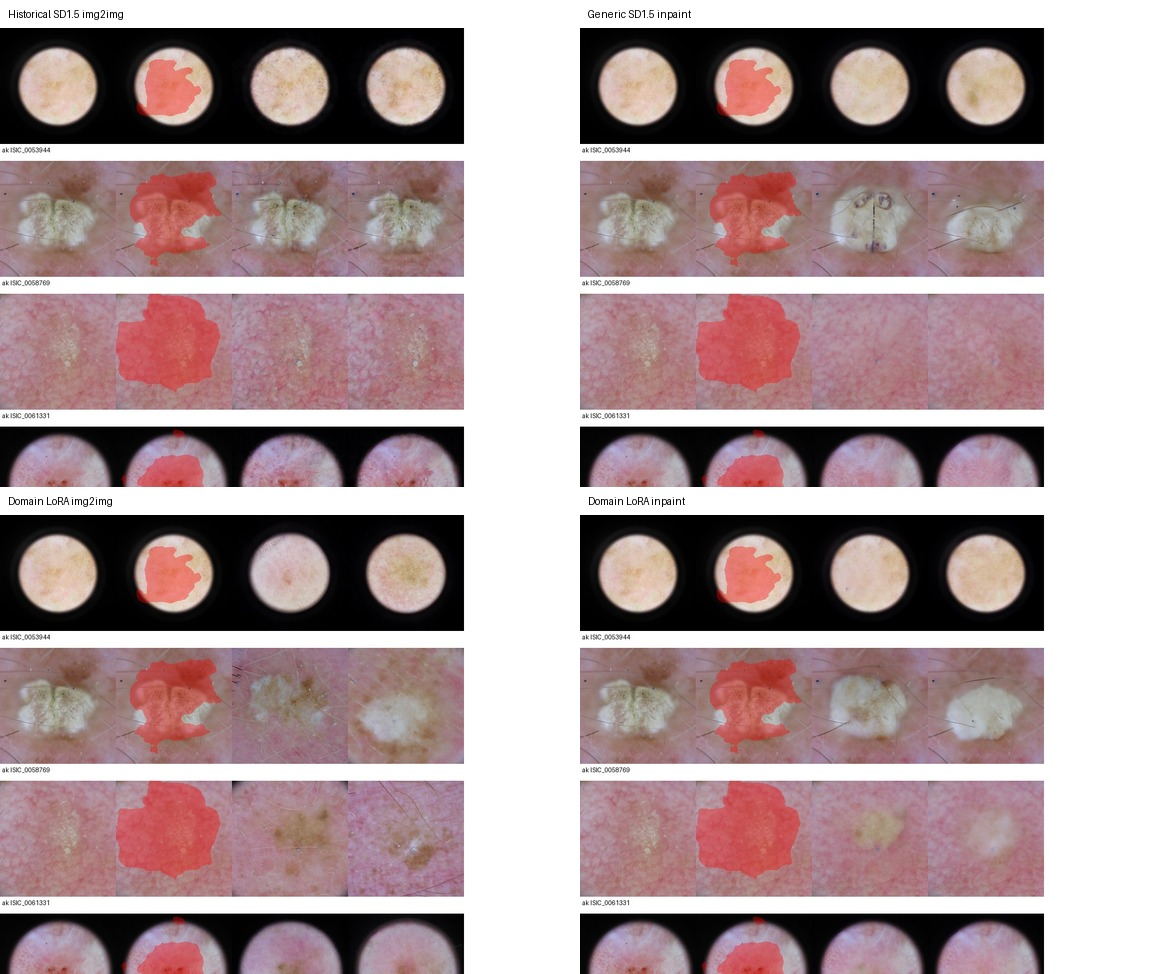
\includegraphics[width=0.80\linewidth]{figures/01_figure_4_generator_examples_internal_audit.jpg}
\caption{TODO: информативная подпись к результату на рис. 1}
\end{figure}

\begin{figure}[h]
\centering
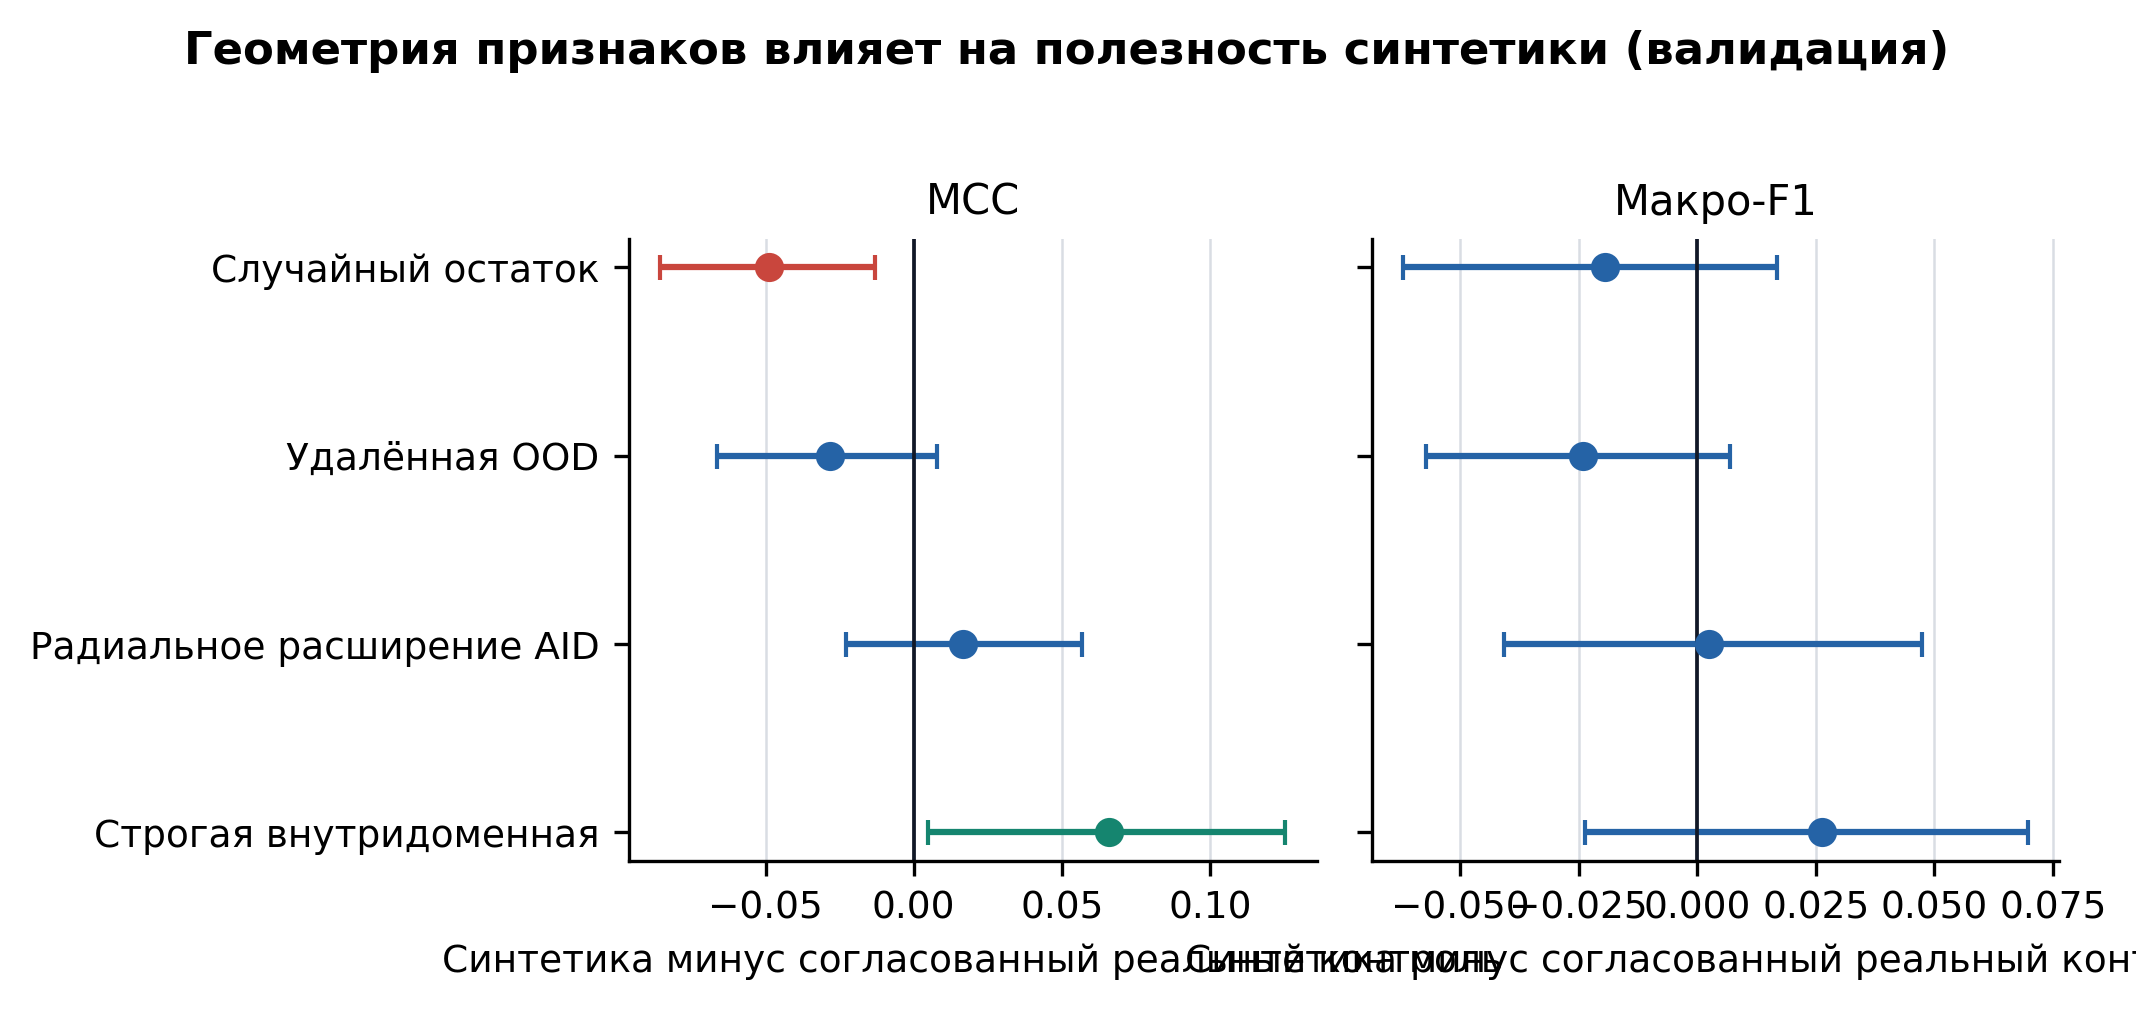
\includegraphics[width=0.80\linewidth]{figures/02_figure_1_stage10_geometry_forest.png}
\caption{TODO: информативная подпись к результату на рис. 2}
\end{figure}

\begin{figure}[h]
\centering
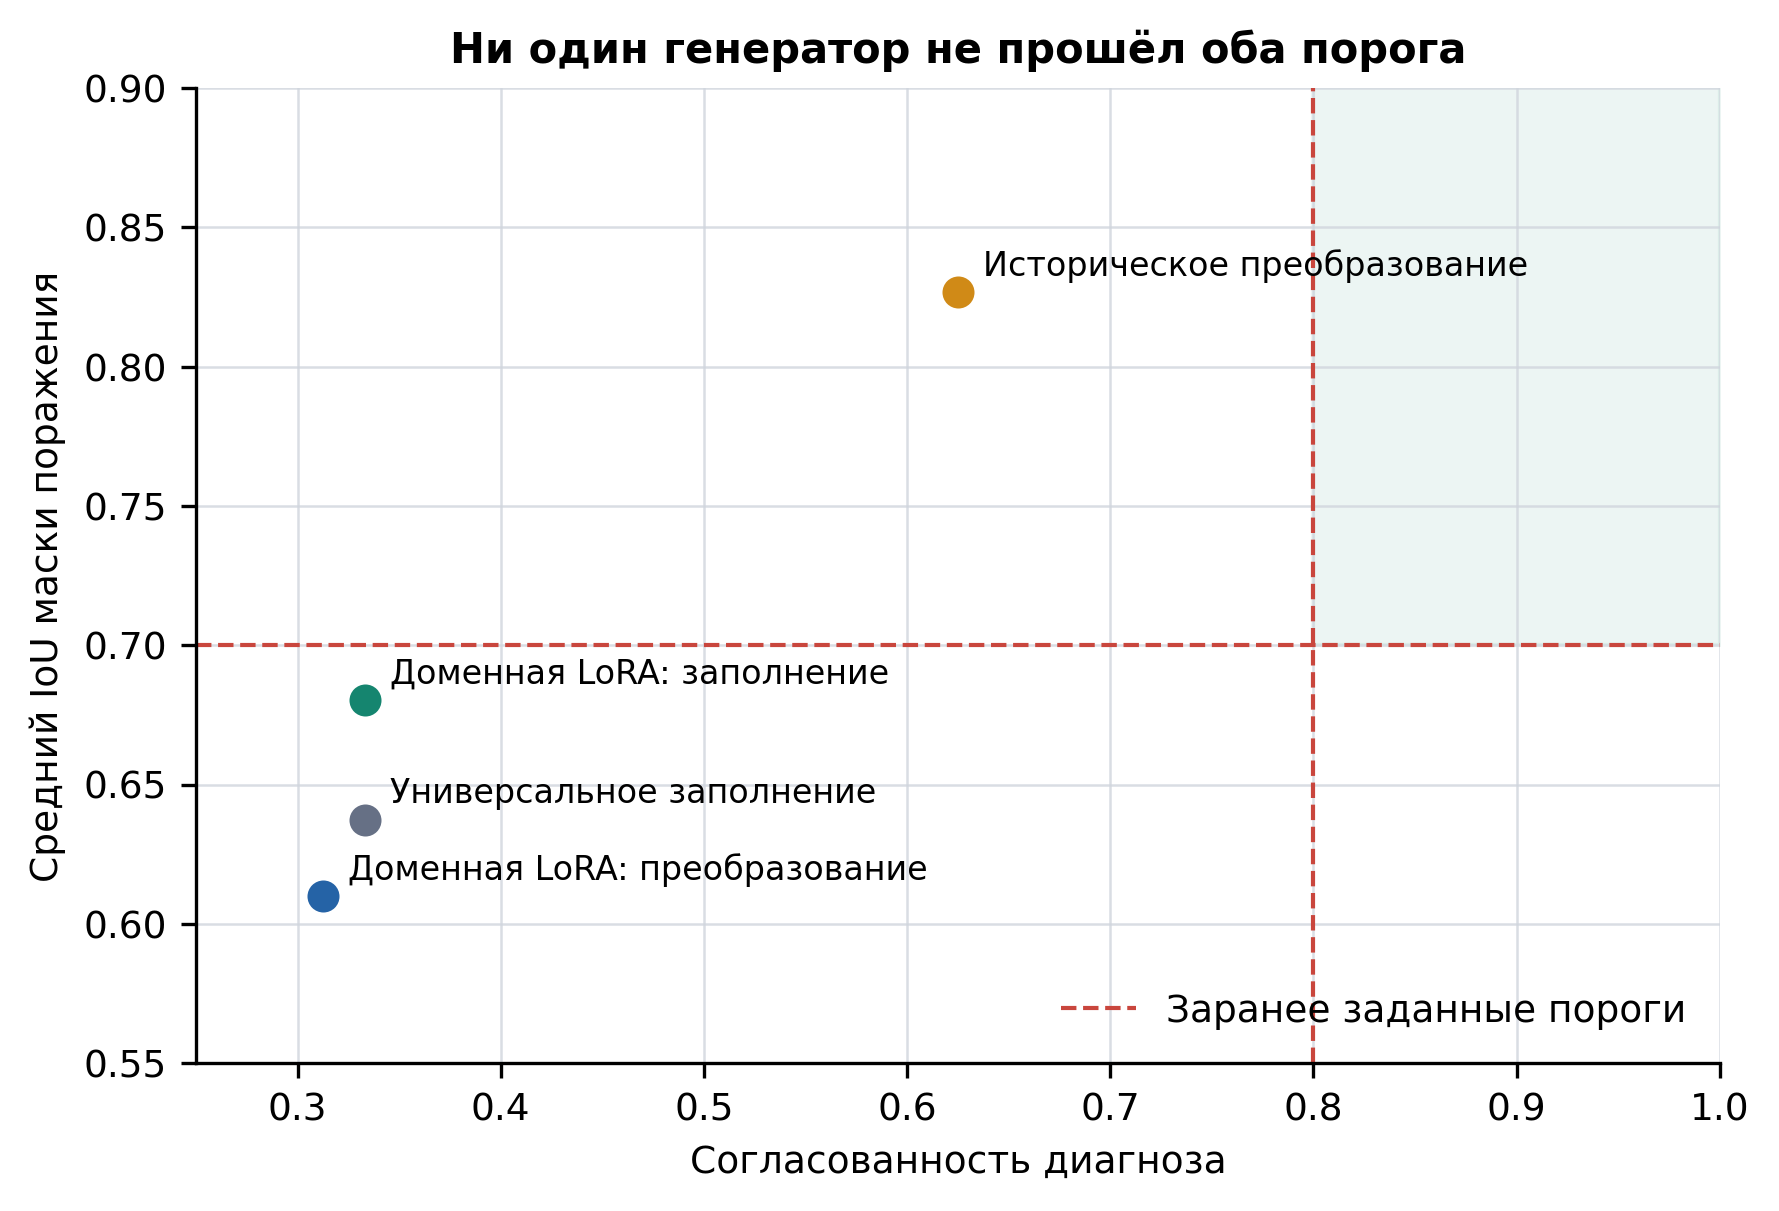
\includegraphics[width=0.80\linewidth]{figures/03_figure_3_generator_qualification.png}
\caption{TODO: информативная подпись к результату на рис. 3}
\end{figure}

\begin{figure}[h]
\centering
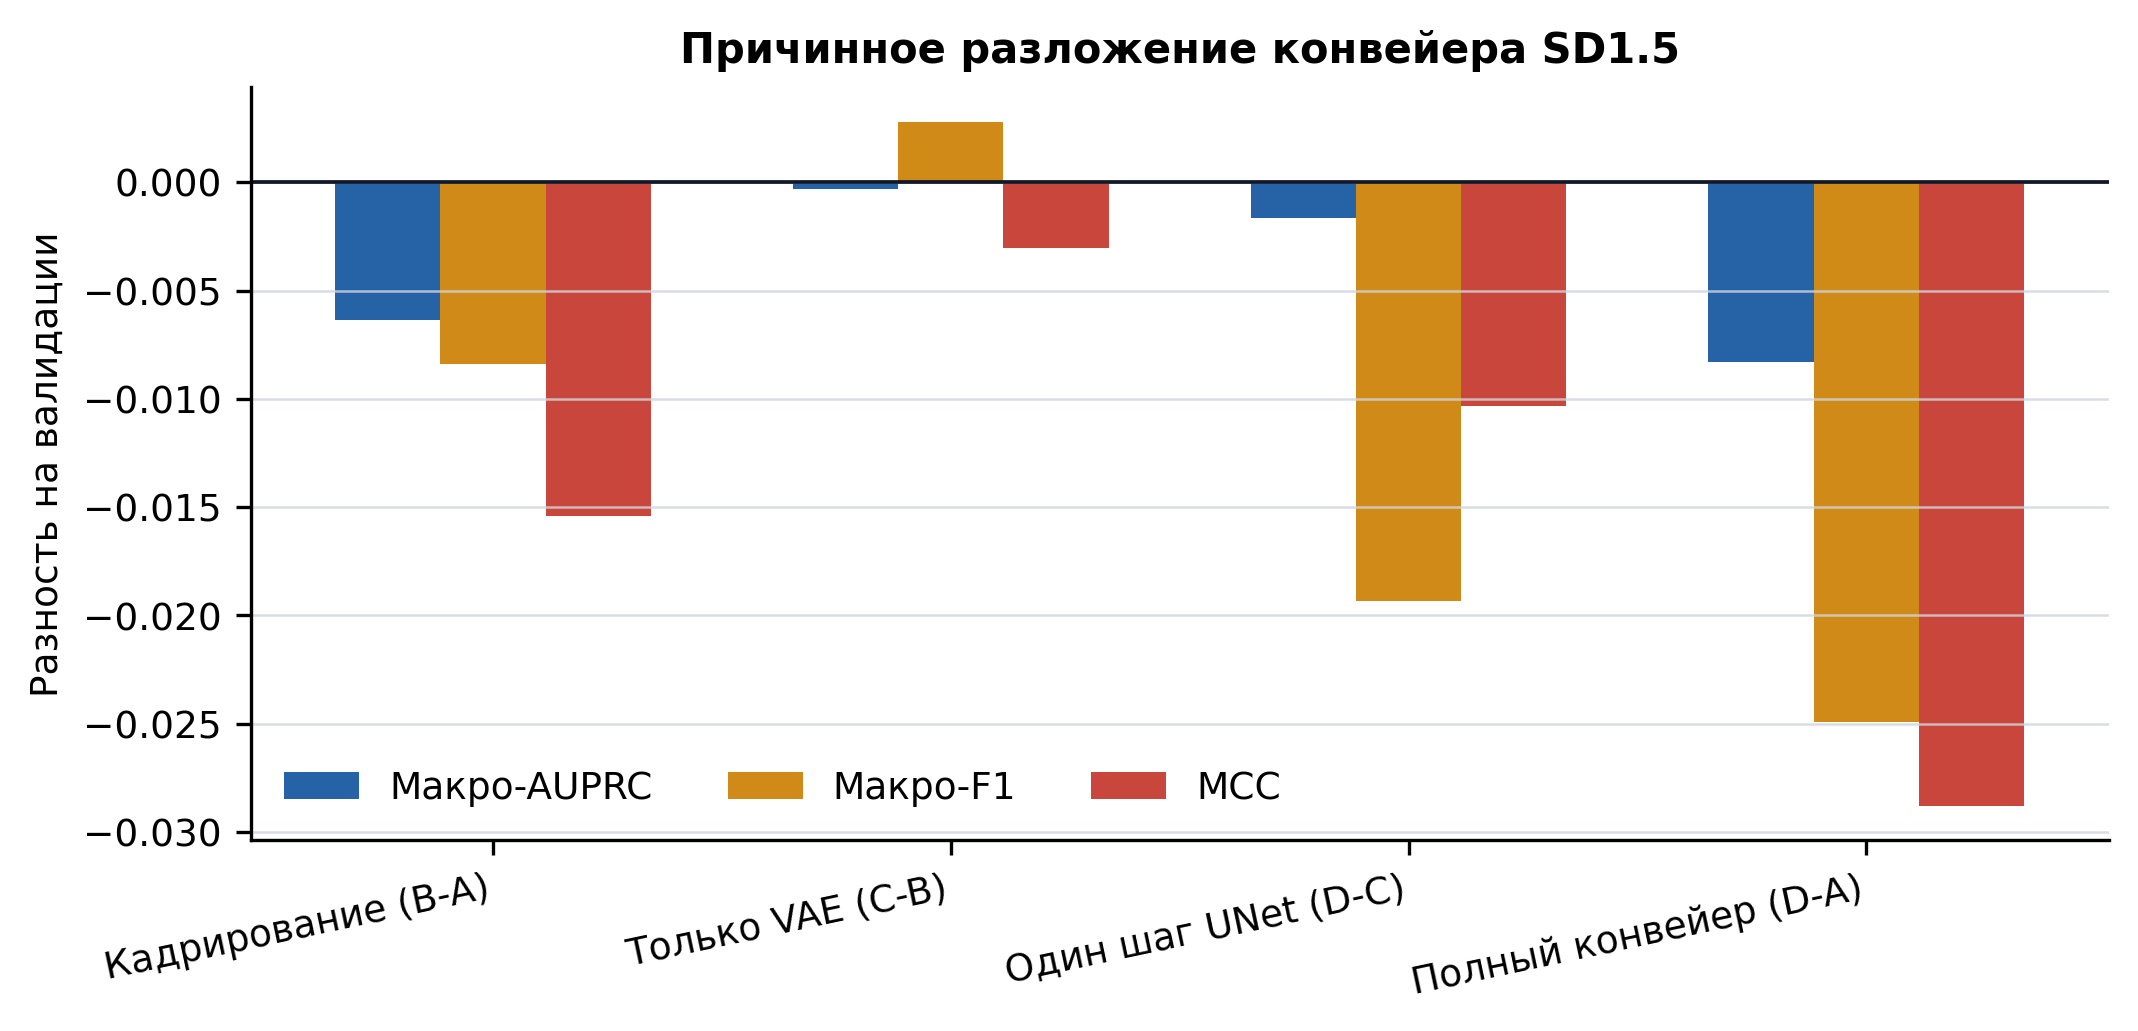
\includegraphics[width=0.80\linewidth]{figures/04_figure_2_stage15a_causal_decomposition.png}
\caption{TODO: информативная подпись к результату на рис. 4}
\end{figure}

\begin{center}
    {\bf 4. Обсуждение}
\end{center}

TODO: обсудить, почему визуальное качество синтетики недостаточно; связать utility с domain gap, coverage, class-conditional geometry и leakage safeguards. Ясно отделить инженерные ограничения от научного вывода.

\begin{center}
    {\bf Заключение}
\end{center}

TODO: 1 абзац с ответом на исследовательский вопрос, 1 абзац с ограничениями, 1 абзац с дальнейшим протоколом. Без новых чисел, которых не было в результатах.

\begin{center}
    {\bf Благодарности}
\end{center}

TODO: указать гранты/инфраструктуру или удалить раздел, если он не нужен.

\begin{center}
    {\bf References}
\end{center}

\begin{enumerate}[topsep=0px,itemsep=-1px]
    \item TODO: оформить источники в порядке цитирования по AMA; DOI обязателен, если есть.
\end{enumerate}

\newpage

\begin{center}
    {\bf Сведения об авторах}
\end{center}

TODO: для каждого автора 10--15 строк: ФИО, степень, звание/должность/место работы, интересы до 15 слов, e-mail, ORCID/web page.

\newpage

\begin{center}
    \section*{TODO: English title}
\end{center}

\begin{center}
TODO: Authors and affiliations in English
\end{center}

\begin{center}
    {\bf Abstract}
\end{center}

TODO: English abstract.

\underline{\it{Keywords}}: TODO.

\underline{\it{Citation}}: TODO.

\begin{center}
    {\bf About authors}
\end{center}

TODO: author information in English.

\end{document}
